\documentclass[11pt]{article}

% ----- geometry & typography
\usepackage[a4paper, margin=1in]{geometry}
\usepackage{microtype}
\usepackage{amsmath, amssymb, amsthm}
\usepackage{mathtools}
\usepackage{xcolor}
\usepackage{hyperref}
\hypersetup{colorlinks=true, linkcolor=blue!50!black, citecolor=blue!50!black, urlcolor=blue!50!black}

% ----- colour palette: cooler & more academic than the relaxation doc
\definecolor{coreblue}{RGB}{40, 70, 130}
\definecolor{coredeep}{RGB}{25, 50, 100}
\definecolor{paradigmA}{RGB}{170, 60, 60}
\definecolor{paradigmB}{RGB}{60, 130, 90}
\definecolor{softA}{RGB}{240, 215, 215}
\definecolor{softB}{RGB}{215, 235, 225}
\definecolor{softblue}{RGB}{215, 225, 240}
\definecolor{accentamber}{RGB}{200, 145, 50}
\definecolor{accentpurple}{RGB}{120, 80, 150}
\definecolor{softpurple}{RGB}{230, 220, 240}
\definecolor{softamber}{RGB}{245, 230, 200}
\definecolor{notegrey}{RGB}{95, 95, 110}
\definecolor{darkgrey}{RGB}{60, 60, 70}

% ----- tikz
\usepackage{tikz}
\usepackage{pgfplots}
\pgfplotsset{compat=1.18}
\usetikzlibrary{
  arrows.meta,
  positioning,
  decorations.pathmorphing,
  decorations.markings,
  decorations.text,
  shapes.geometric,
  shapes.misc,
  fit,
  backgrounds,
  calc,
  patterns,
  intersections
}

\title{Figures for the Structural Paradigm Model\\[0.2em]\large Working sketches}
\author{}
\date{\today}

\begin{document}
\maketitle

\noindent\textit{\textcolor{notegrey}{This document collects candidate figures for the structural version of the paradigm-dynamics paper. Each figure is paired with a note describing what work it does in the argument, where in the paper it would sit, and what it would have to be replaced or extended with once simulation results are available. The figures are designed to make the structural-versus-scalar contrast visible, to display the carry-over property as message propagation through a precision-weighted network, and to render the BMR move as a transition between corner configurations of a continuous precision space.}}

%==============================================================
\section*{Figure 1: The paradigm as a structured object}
%==============================================================

\textit{Where it sits.} Section 1 or early section 2 — wherever the paper first introduces the structural representation of the paradigm. This is the figure that says, before any equations, that the paradigm is not a scalar.

\textit{What work it does.} It contrasts, side by side, two representations of the same theoretical commitment. On the left, the paradigm as it appears in the scalar treatment: a single variable taking values in a discrete set. On the right, the paradigm as a structured Bayes net of interdependent commitments. The right-hand panel is the object the paper is actually about.

\begin{center}
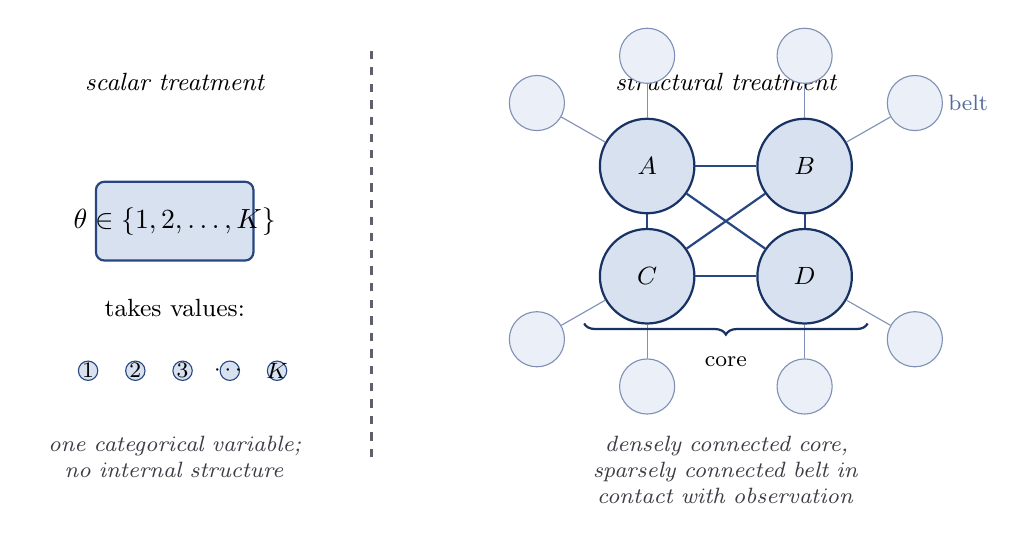
\begin{tikzpicture}[scale=1]

  % ---------- LEFT PANEL: scalar paradigm ----------
  \begin{scope}[xshift=0cm]
    \node[font=\small\itshape, anchor=north] at (1.5, 4.5) {scalar treatment};

    % the variable
    \draw[thick, coreblue, fill=softblue, rounded corners=3pt] (0.5, 2) rectangle (2.5, 3);
    \node at (1.5, 2.5) {$\theta \in \{1, 2, \ldots, K\}$};

    % discrete values shown below
    \node[font=\small] at (1.5, 1.4) {takes values:};
    \foreach \x/\v in {0.4/$1$, 1/$2$, 1.6/$3$, 2.2/$\cdots$, 2.8/$K$} {
      \draw[coreblue, fill=softblue] (\x, 0.6) circle (3.5pt);
      \node[font=\footnotesize] at (\x, 0.6) {\v};
    }

    \node[font=\footnotesize\itshape, anchor=north, text width=3.5cm, align=center, text=darkgrey]
      at (1.5, -0.1) {one categorical variable;\\ no internal structure};
  \end{scope}

  % divider
  \draw[thick, dashed, notegrey] (4, -0.5) -- (4, 4.7);

  % ---------- RIGHT PANEL: structured paradigm ----------
  \begin{scope}[xshift=4.5cm]
    \node[font=\small\itshape, anchor=north] at (4, 4.5) {structural treatment};

    % core nodes (densely connected centre)
    \node[circle, draw=coredeep, thick, fill=softblue, minimum size=12mm, font=\small] (A) at (3, 3.2) {$A$};
    \node[circle, draw=coredeep, thick, fill=softblue, minimum size=12mm, font=\small] (B) at (5, 3.2) {$B$};
    \node[circle, draw=coredeep, thick, fill=softblue, minimum size=12mm, font=\small] (C) at (3, 1.8) {$C$};
    \node[circle, draw=coredeep, thick, fill=softblue, minimum size=12mm, font=\small] (D) at (5, 1.8) {$D$};

    % dense core connections
    \draw[thick, coreblue] (A) -- (B);
    \draw[thick, coreblue] (A) -- (C);
    \draw[thick, coreblue] (A) -- (D);
    \draw[thick, coreblue] (B) -- (C);
    \draw[thick, coreblue] (B) -- (D);
    \draw[thick, coreblue] (C) -- (D);

    % belt nodes (lighter, sparser)
    \node[circle, draw=coreblue!60, fill=softblue!50, minimum size=7mm, font=\footnotesize] (b1) at (1.6, 4.0) {};
    \node[circle, draw=coreblue!60, fill=softblue!50, minimum size=7mm, font=\footnotesize] (b2) at (6.4, 4.0) {};
    \node[circle, draw=coreblue!60, fill=softblue!50, minimum size=7mm, font=\footnotesize] (b3) at (1.6, 1.0) {};
    \node[circle, draw=coreblue!60, fill=softblue!50, minimum size=7mm, font=\footnotesize] (b4) at (6.4, 1.0) {};
    \node[circle, draw=coreblue!60, fill=softblue!50, minimum size=7mm, font=\footnotesize] (b5) at (3, 0.4) {};
    \node[circle, draw=coreblue!60, fill=softblue!50, minimum size=7mm, font=\footnotesize] (b6) at (5, 0.4) {};
    \node[circle, draw=coreblue!60, fill=softblue!50, minimum size=7mm, font=\footnotesize] (b7) at (3, 4.6) {};
    \node[circle, draw=coreblue!60, fill=softblue!50, minimum size=7mm, font=\footnotesize] (b8) at (5, 4.6) {};

    % belt-to-core edges (thinner)
    \draw[coreblue!60] (b1) -- (A);
    \draw[coreblue!60] (b2) -- (B);
    \draw[coreblue!60] (b3) -- (C);
    \draw[coreblue!60] (b4) -- (D);
    \draw[coreblue!60] (b5) -- (C);
    \draw[coreblue!60] (b6) -- (D);
    \draw[coreblue!60] (b7) -- (A);
    \draw[coreblue!60] (b8) -- (B);

    % labels
    \draw[decorate, decoration={brace, amplitude=4pt, mirror}, thick, coredeep]
      (2.2, 1.2) -- (5.8, 1.2);
    \node[font=\footnotesize, anchor=north] at (4, 0.9) {core};

    \node[font=\footnotesize, anchor=west, text=coreblue!80] at (6.7, 4.0) {belt};

    \node[font=\footnotesize\itshape, anchor=north, text width=5cm, align=center, text=darkgrey]
      at (4, -0.1) {densely connected core,\\ sparsely connected belt in contact with observation};
  \end{scope}

\end{tikzpicture}
\end{center}

\noindent\textit{\textcolor{notegrey}{The visual asymmetry between the two panels is doing the rhetorical work. Left is small and tidy and obviously inadequate to the conceptual job a paradigm has to do; right is structured and rich and visibly carries inferential dependency. The core-belt distinction is shown geometrically (dense centre, sparse periphery) but not yet quantitatively — the precision-weighted version comes in Figure 3.}}

\newpage
%==============================================================
\section*{Figure 2: The carry-over property}
%==============================================================

\textit{Where it sits.} Section 3 or 4, where the paper introduces structural utility and explains why paradigm revision is expensive. This is the figure that makes the carry-over property visible — the central conceptual move that distinguishes the structural model from the scalar one.

\textit{What work it does.} It shows a node value changing in the structured paradigm, and the resulting wave of revision propagating outward through the inferentially-connected commitments. The point is that you cannot move a core node without forcing reinterpretation of everything that depends on it; this is the structural counterpart of Kuhnian incommensurability, made literal as message propagation.

\begin{center}
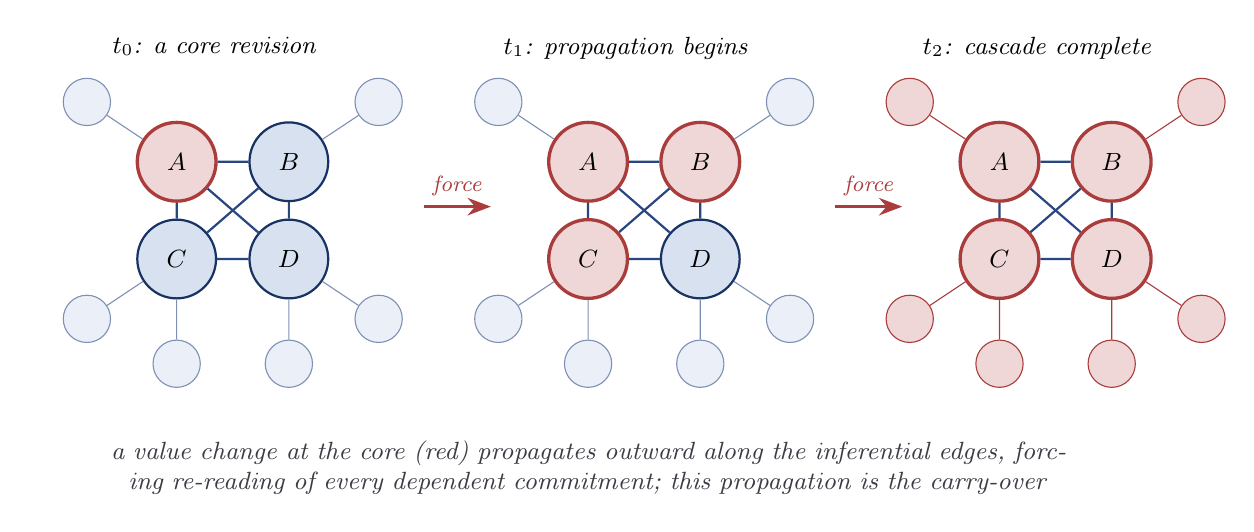
\begin{tikzpicture}[scale=0.95]

  % three time slices showing the cascade
  \foreach \tx/\tlab/\activeA/\activeB/\activeC/\activeD/\activeBelt in {
    0/$t_0$: a core revision/1/0/0/0/0,
    5.5/$t_1$: propagation begins/1/1/1/0/0,
    11/$t_2$: cascade complete/1/1/1/1/1
  } {
    \begin{scope}[xshift=\tx cm]
      \node[font=\small\itshape, anchor=north] at (2, 5.2) {\tlab};

      % core nodes - colour depends on whether revised
      \ifnum\activeA=1
        \node[circle, draw=paradigmA, very thick, fill=softA, minimum size=10mm, font=\small] (A) at (1.5, 3.4) {$A$};
      \else
        \node[circle, draw=coredeep, thick, fill=softblue, minimum size=10mm, font=\small] (A) at (1.5, 3.4) {$A$};
      \fi
      \ifnum\activeB=1
        \node[circle, draw=paradigmA, very thick, fill=softA, minimum size=10mm, font=\small] (B) at (3, 3.4) {$B$};
      \else
        \node[circle, draw=coredeep, thick, fill=softblue, minimum size=10mm, font=\small] (B) at (3, 3.4) {$B$};
      \fi
      \ifnum\activeC=1
        \node[circle, draw=paradigmA, very thick, fill=softA, minimum size=10mm, font=\small] (C) at (1.5, 2.1) {$C$};
      \else
        \node[circle, draw=coredeep, thick, fill=softblue, minimum size=10mm, font=\small] (C) at (1.5, 2.1) {$C$};
      \fi
      \ifnum\activeD=1
        \node[circle, draw=paradigmA, very thick, fill=softA, minimum size=10mm, font=\small] (D) at (3, 2.1) {$D$};
      \else
        \node[circle, draw=coredeep, thick, fill=softblue, minimum size=10mm, font=\small] (D) at (3, 2.1) {$D$};
      \fi

      % core edges
      \draw[thick, coreblue] (A) -- (B);
      \draw[thick, coreblue] (A) -- (C);
      \draw[thick, coreblue] (A) -- (D);
      \draw[thick, coreblue] (B) -- (C);
      \draw[thick, coreblue] (B) -- (D);
      \draw[thick, coreblue] (C) -- (D);

      % belt nodes
      \ifnum\activeBelt=1
        \def\beltcolour{paradigmA}
        \def\beltfill{softA}
      \else
        \def\beltcolour{coreblue!60}
        \def\beltfill{softblue!50}
      \fi
      \node[circle, draw=\beltcolour, fill=\beltfill, minimum size=6mm, font=\footnotesize] (b1) at (0.3, 4.2) {};
      \node[circle, draw=\beltcolour, fill=\beltfill, minimum size=6mm, font=\footnotesize] (b2) at (4.2, 4.2) {};
      \node[circle, draw=\beltcolour, fill=\beltfill, minimum size=6mm, font=\footnotesize] (b3) at (0.3, 1.3) {};
      \node[circle, draw=\beltcolour, fill=\beltfill, minimum size=6mm, font=\footnotesize] (b4) at (4.2, 1.3) {};
      \node[circle, draw=\beltcolour, fill=\beltfill, minimum size=6mm, font=\footnotesize] (b5) at (1.5, 0.7) {};
      \node[circle, draw=\beltcolour, fill=\beltfill, minimum size=6mm, font=\footnotesize] (b6) at (3, 0.7) {};

      % belt edges
      \draw[\beltcolour] (b1) -- (A);
      \draw[\beltcolour] (b2) -- (B);
      \draw[\beltcolour] (b3) -- (C);
      \draw[\beltcolour] (b4) -- (D);
      \draw[\beltcolour] (b5) -- (C);
      \draw[\beltcolour] (b6) -- (D);
    \end{scope}
  }

  % propagation arrows between time slices
  \draw[->, very thick, paradigmA, >=Stealth] (4.8, 2.8) -- (5.7, 2.8)
    node[midway, above, font=\footnotesize\itshape] {force};
  \draw[->, very thick, paradigmA, >=Stealth] (10.3, 2.8) -- (11.2, 2.8)
    node[midway, above, font=\footnotesize\itshape] {force};

  % bottom label
  \node[font=\small\itshape, anchor=north, text=darkgrey, text width=14cm, align=center]
    at (7, -0.2) {a value change at the core (red) propagates outward along the inferential edges, forcing re-reading of every dependent commitment; this propagation is the carry-over};
\end{tikzpicture}
\end{center}

\noindent\textit{\textcolor{notegrey}{This figure is the most important one in the paper because it makes the carry-over property — the thing the scalar treatment cannot represent — visually unmistakable. The colour gradient (one node red, then several, then all) shows the cascade as it actually runs through the message-passing dynamics. The arrows between panels are labelled ``force'' to emphasize that the propagation is not a choice but a consequence of the structural commitments. In the published version this would be paired with the relevant equation for the precision-weighted update, but the figure should be readable without the maths.}}

\newpage
%==============================================================
\section*{Figure 3: Conservatism falls out of structure (not assignment)}
%==============================================================

\textit{Where it sits.} Section 3 or 4, immediately after the carry-over figure. This figure makes precise what was visual in Figure 2: the differential cost of revising different nodes is not assigned but derives from each node's structural position.

\textit{What work it does.} It shows a node-by-node breakdown of the conservatism $\lambda_i$ at each position in the network, with the value at each node derived from its connectivity rather than imposed. The colour intensity encodes $\lambda_i$. The reader sees, without equations, that the core's high conservatism is structurally derived rather than parametrically asserted.

\begin{center}
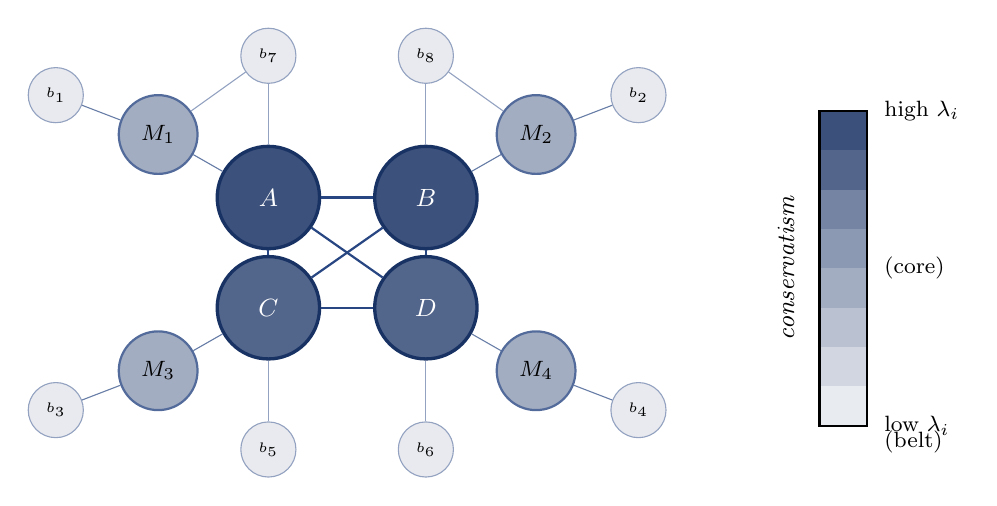
\begin{tikzpicture}[scale=1]
  % the network, with node fill encoding lambda_i

  % core nodes - high lambda (dark)
  \node[circle, draw=coredeep, very thick, fill=coredeep!85, minimum size=13mm, font=\small, text=white] (A) at (3, 3.4) {$A$};
  \node[circle, draw=coredeep, very thick, fill=coredeep!85, minimum size=13mm, font=\small, text=white] (B) at (5, 3.4) {$B$};
  \node[circle, draw=coredeep, very thick, fill=coredeep!75, minimum size=13mm, font=\small, text=white] (C) at (3, 2.0) {$C$};
  \node[circle, draw=coredeep, very thick, fill=coredeep!75, minimum size=13mm, font=\small, text=white] (D) at (5, 2.0) {$D$};

  % core-core edges
  \draw[thick, coreblue] (A) -- (B);
  \draw[thick, coreblue] (A) -- (C);
  \draw[thick, coreblue] (A) -- (D);
  \draw[thick, coreblue] (B) -- (C);
  \draw[thick, coreblue] (B) -- (D);
  \draw[thick, coreblue] (C) -- (D);

  % intermediate-shell nodes - moderate lambda
  \node[circle, draw=coreblue!80, thick, fill=coredeep!40, minimum size=10mm, font=\footnotesize] (m1) at (1.6, 4.2) {$M_1$};
  \node[circle, draw=coreblue!80, thick, fill=coredeep!40, minimum size=10mm, font=\footnotesize] (m2) at (6.4, 4.2) {$M_2$};
  \node[circle, draw=coreblue!80, thick, fill=coredeep!40, minimum size=10mm, font=\footnotesize] (m3) at (1.6, 1.2) {$M_3$};
  \node[circle, draw=coreblue!80, thick, fill=coredeep!40, minimum size=10mm, font=\footnotesize] (m4) at (6.4, 1.2) {$M_4$};

  % belt nodes - low lambda (light)
  \node[circle, draw=coreblue!50, fill=coredeep!10, minimum size=7mm, font=\tiny] (b1) at (0.3, 4.7) {$b_1$};
  \node[circle, draw=coreblue!50, fill=coredeep!10, minimum size=7mm, font=\tiny] (b2) at (7.7, 4.7) {$b_2$};
  \node[circle, draw=coreblue!50, fill=coredeep!10, minimum size=7mm, font=\tiny] (b3) at (0.3, 0.7) {$b_3$};
  \node[circle, draw=coreblue!50, fill=coredeep!10, minimum size=7mm, font=\tiny] (b4) at (7.7, 0.7) {$b_4$};
  \node[circle, draw=coreblue!50, fill=coredeep!10, minimum size=7mm, font=\tiny] (b5) at (3, 0.2) {$b_5$};
  \node[circle, draw=coreblue!50, fill=coredeep!10, minimum size=7mm, font=\tiny] (b6) at (5, 0.2) {$b_6$};
  \node[circle, draw=coreblue!50, fill=coredeep!10, minimum size=7mm, font=\tiny] (b7) at (3, 5.2) {$b_7$};
  \node[circle, draw=coreblue!50, fill=coredeep!10, minimum size=7mm, font=\tiny] (b8) at (5, 5.2) {$b_8$};

  % edges from belt to intermediate, intermediate to core
  \draw[coreblue!70] (b1) -- (m1);
  \draw[coreblue!70] (b2) -- (m2);
  \draw[coreblue!70] (b3) -- (m3);
  \draw[coreblue!70] (b4) -- (m4);
  \draw[coreblue!50] (b5) -- (C);
  \draw[coreblue!50] (b6) -- (D);
  \draw[coreblue!50] (b7) -- (A);
  \draw[coreblue!50] (b8) -- (B);
  \draw[coreblue!70] (m1) -- (A);
  \draw[coreblue!70] (m2) -- (B);
  \draw[coreblue!70] (m3) -- (C);
  \draw[coreblue!70] (m4) -- (D);
  \draw[coreblue!50] (m1) -- (b7);
  \draw[coreblue!50] (m2) -- (b8);

  % colour bar / legend on the right
  \begin{scope}[xshift=10cm, yshift=0.5cm]
    % gradient bar
    \foreach \y/\op in {0/10, 0.5/20, 1/30, 1.5/40, 2/50, 2.5/60, 3/75, 3.5/85} {
      \fill[coredeep, opacity=0.01*\op] (0, \y) rectangle (0.6, \y+0.5);
    }
    \draw[thick] (0, 0) rectangle (0.6, 4);
    \node[font=\footnotesize, anchor=west] at (0.7, 4) {high $\lambda_i$};
    \node[font=\footnotesize, anchor=west] at (0.7, 2) {(core)};
    \node[font=\footnotesize, anchor=west] at (0.7, 0) {low $\lambda_i$};
    \node[font=\footnotesize, anchor=west] at (0.7, -0.2) {(belt)};
    \node[font=\small\itshape, anchor=south, rotate=90] at (-0.2, 2) {conservatism};
  \end{scope}

\end{tikzpicture}
\end{center}

\noindent\textit{\textcolor{notegrey}{The figure encodes $\lambda_i$ by colour saturation. The point is that no $\lambda$ is assigned: each node's conservatism is the precision-weighted KL cost of moving its value through the message-passing on the network, which is high in the core because the core has many downstream dependencies and low in the belt because the belt has few. The figure also introduces an intermediate shell of $M_i$ nodes (slightly less core than $A$--$D$) to make the gradient continuous rather than binary, which is important for the BMR-style continuous structure-learning that comes in Figure 5.}}

\newpage
%==============================================================
\section*{Figure 4: BMR as precision corner navigation}
%==============================================================

\textit{Where it sits.} Section 4 or 5, where the paper introduces Bayesian model reduction as the principled treatment of structural inference. This figure pulls double duty: it explains BMR visually for readers who don't know it, and it shows that the discrete corners of the precision space (sharp Bayes-net topologies) are recoverable as limits of a continuous interior (smoothly weighted partial edges).

\textit{What work it does.} It renders the BMR move as navigation through a continuous precision space whose corners are the discrete Bayes-net topologies. A trajectory through this space is what the agent does when it considers structural revisions.

\begin{center}
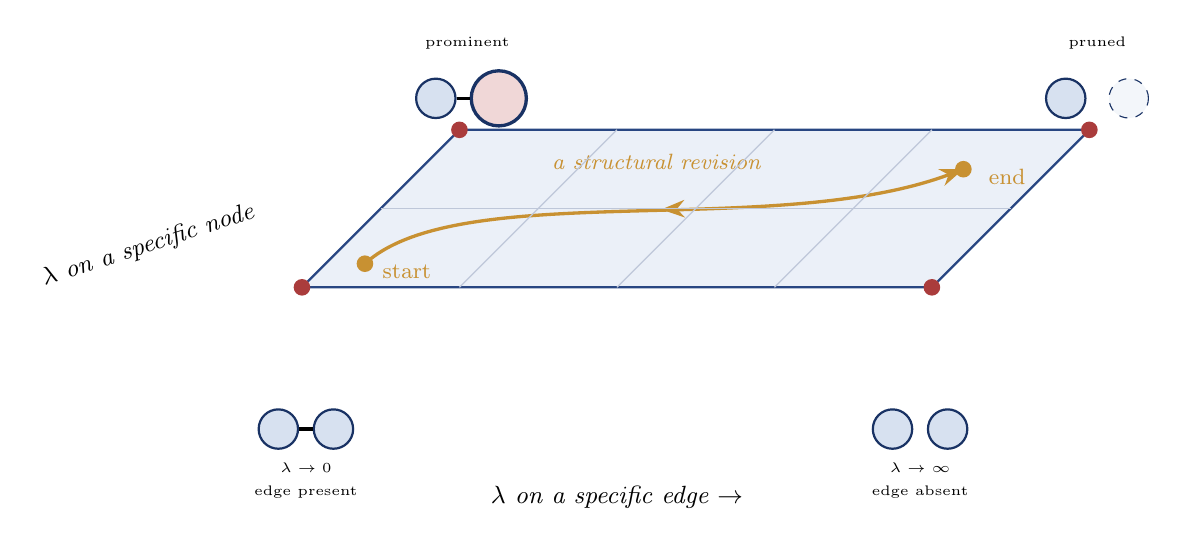
\begin{tikzpicture}[scale=1]

  % the precision square / cube schematic
  \draw[thick, coreblue, fill=softblue!50] (0, 0) -- (8, 0) -- (10, 2) -- (2, 2) -- cycle;

  % corner labels with mini-networks
  % bottom-left: edge fully present (low lambda)
  \begin{scope}[xshift=-0.3cm, yshift=-1.8cm]
    \node[circle, draw=coredeep, thick, fill=softblue, minimum size=5mm, font=\tiny] (a1) at (0, 0) {};
    \node[circle, draw=coredeep, thick, fill=softblue, minimum size=5mm, font=\tiny] (a2) at (0.7, 0) {};
    \draw[line width=1.5pt] (a1) -- (a2);
    \node[font=\tiny, anchor=north] at (0.35, -0.3) {$\lambda \to 0$};
    \node[font=\tiny, anchor=north] at (0.35, -0.6) {edge present};
  \end{scope}

  % bottom-right: edge absent (high lambda)
  \begin{scope}[xshift=7.5cm, yshift=-1.8cm]
    \node[circle, draw=coredeep, thick, fill=softblue, minimum size=5mm, font=\tiny] (a3) at (0, 0) {};
    \node[circle, draw=coredeep, thick, fill=softblue, minimum size=5mm, font=\tiny] (a4) at (0.7, 0) {};
    % no edge
    \node[font=\tiny, anchor=north] at (0.35, -0.3) {$\lambda \to \infty$};
    \node[font=\tiny, anchor=north] at (0.35, -0.6) {edge absent};
  \end{scope}

  % top-left: large precision (node prominent)
  \begin{scope}[xshift=1.7cm, yshift=2.4cm]
    \node[circle, draw=coredeep, thick, fill=softblue, minimum size=5mm, font=\tiny] (a5) at (0, 0) {};
    \node[circle, draw=coredeep, very thick, fill=softA, minimum size=7mm, font=\tiny] (a6) at (0.8, 0) {};
    \draw[line width=1.2pt] (a5) -- (a6);
    \node[font=\tiny, anchor=south] at (0.4, 0.5) {prominent};
  \end{scope}

  % top-right
  \begin{scope}[xshift=9.7cm, yshift=2.4cm]
    \node[circle, draw=coredeep, thick, fill=softblue, minimum size=5mm, font=\tiny] (a7) at (0, 0) {};
    \node[circle, draw=coredeep, dashed, fill=softblue!30, minimum size=5mm, font=\tiny] (a8) at (0.8, 0) {};
    \node[font=\tiny, anchor=south] at (0.4, 0.5) {pruned};
  \end{scope}

  % corner markers
  \fill[paradigmA] (0, 0) circle (3pt);
  \fill[paradigmA] (8, 0) circle (3pt);
  \fill[paradigmA] (2, 2) circle (3pt);
  \fill[paradigmA] (10, 2) circle (3pt);

  % axis labels
  \node[font=\small\itshape, anchor=north] at (4, -2.4) {$\lambda$ on a specific edge $\to$};
  \node[font=\small\itshape, anchor=east, rotate=18] at (-0.5, 1) {$\lambda$ on a specific node};

  % trajectory through the space
  \draw[->, very thick, accentamber, >=Stealth,
        decoration={markings, mark=at position 0.5 with {\arrowreversed{>}}}, postaction={decorate}]
    (0.8, 0.3) .. controls (2, 1.4) and (6, 0.6) .. (8.4, 1.5);

  % start and end markers on trajectory
  \fill[accentamber] (0.8, 0.3) circle (3pt);
  \node[font=\footnotesize, accentamber, anchor=west] at (0.9, 0.2) {start};
  \fill[accentamber] (8.4, 1.5) circle (3pt);
  \node[font=\footnotesize, accentamber, anchor=west] at (8.6, 1.4) {end};

  % label the trajectory
  \node[font=\footnotesize\itshape, accentamber] at (4.5, 1.6) {a structural revision};

  % interior shading suggesting continuous space
  \foreach \x in {2, 4, 6} {
    \draw[coreblue!30, thin] (\x, 0) -- (\x+2, 2);
  }
  \draw[coreblue!30, thin] (1, 1) -- (9, 1);

\end{tikzpicture}
\end{center}

\bigskip
\bigskip

\noindent\textit{\textcolor{notegrey}{The figure shows the precision space as a two-dimensional patch (one axis per varied precision; in reality the space is high-dimensional). The four corners are discrete Bayes-net topologies, distinguished by which precisions are at infinity (edges absent) and which are at zero (edges present). The interior is the continuous relaxation: partial edges, soft structural commitments, smoothly varying conservatism. The orange trajectory is a structural revision in progress — the agent gradually shifts its precisions, traversing the interior of the space, without ever needing to make a discrete jump. This is the relaxation move from the previous document, applied here to the structural-inference problem the paradigm paper has to solve. In the body of the paper this figure would replace the discrete "model selection" framing with the continuous "precision navigation" framing, which is what enables the fine-grained phase-transition dynamics the structural model produces.}}

\newpage
%==============================================================
\section*{Figure 5: Scalar cascade versus structural phase transition}
%==============================================================

\textit{Where it sits.} Section 6 or 7, where the paper presents the central empirical contrast. This is the headline result figure: the qualitative difference between what the scalar treatment produces and what the structural treatment produces.

\textit{What work it does.} It puts on the same axes the order parameter trajectories from both treatments. The scalar version produces a sharp cascade (sigmoid switch at a threshold). The structural version produces a sequence of finer-grained step-like transitions corresponding to the gradual reorganisation of the precision-weighted network, with a different aggregate signature.

\begin{center}
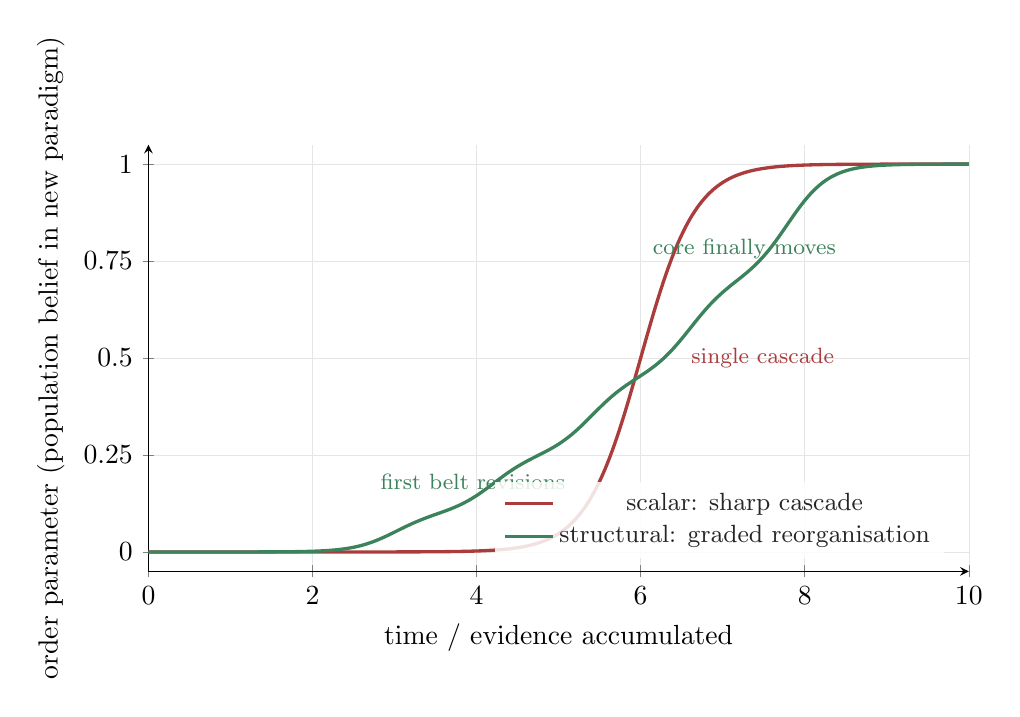
\begin{tikzpicture}
\begin{axis}[
  width=12cm, height=7cm,
  xlabel={time / evidence accumulated},
  ylabel={order parameter (population belief in new paradigm)},
  xmin=0, xmax=10, ymin=-0.05, ymax=1.05,
  xtick={0, 2, 4, 6, 8, 10},
  ytick={0, 0.25, 0.5, 0.75, 1},
  grid=major,
  grid style={gray!20, very thin},
  legend pos=south east,
  legend style={font=\small, draw=none, fill=white, fill opacity=0.85},
  axis lines=left,
  every axis plot/.append style={very thick},
]

  % scalar: sharp sigmoid cascade
  \addplot[paradigmA, smooth, samples=200, domain=0:10]
    {1/(1+exp(-3*(x-6)))};
  \addlegendentry{scalar: sharp cascade}

  % structural: stepped continuous transition (multiple smaller steps)
  \addplot[paradigmB, smooth, samples=400, domain=0:10]
    {0.1/(1+exp(-4*(x-3.0))) +
     0.15/(1+exp(-4*(x-4.2))) +
     0.2/(1+exp(-4*(x-5.4))) +
     0.25/(1+exp(-4*(x-6.6))) +
     0.3/(1+exp(-4*(x-7.8)))};
  \addlegendentry{structural: graded reorganisation}

  % annotation arrows
  \node[font=\footnotesize, paradigmA, anchor=west] at (axis cs:6.5, 0.5) {single cascade};
  \node[font=\footnotesize, paradigmB, anchor=east] at (axis cs:5.2, 0.18) {first belt revisions};
  \node[font=\footnotesize, paradigmB, anchor=east] at (axis cs:8.5, 0.78) {core finally moves};

\end{axis}
\end{tikzpicture}
\end{center}

\noindent\textit{\textcolor{notegrey}{The crucial difference between the two curves is not where they end (both go to 1) but the shape of the approach. The red scalar curve has one inflection point because there is only one variable to flip. The green structural curve has multiple smaller transitions corresponding to successive structural revisions — early ones in the belt are cheap and happen first, later ones in the core are expensive and happen last. The aggregate signature is a graded approach with internal structure, and the internal structure is empirically measurable. This figure is the one that David's scalar simulations alone cannot produce; the structural extension is precisely what makes the green curve a thing to plot. The figure should be replaced with actual simulation output once the structural model is implemented, but the schematic version captures what the result is expected to look like.}}

\newpage
%==============================================================
\section*{Figure 6: Multi-agent coupling with structured beliefs}
%==============================================================

\textit{Where it sits.} Section 5 or 6, where the paper moves from the single-agent to the multi-agent setting. This figure shows the full multi-agent object: each agent carries a structured paradigm network, and inter-agent communication propagates candidate structural revisions across precision-weighted trust channels.

\textit{What work it does.} It makes visible the move that the document we critiqued missed entirely: the scalar trust matrix $T$ acting on scalar paradigm beliefs gets replaced by structured belief exchange, where what each agent emits is a candidate structural revision and what each agent receives is filtered through precision on the trust channel.

\begin{center}
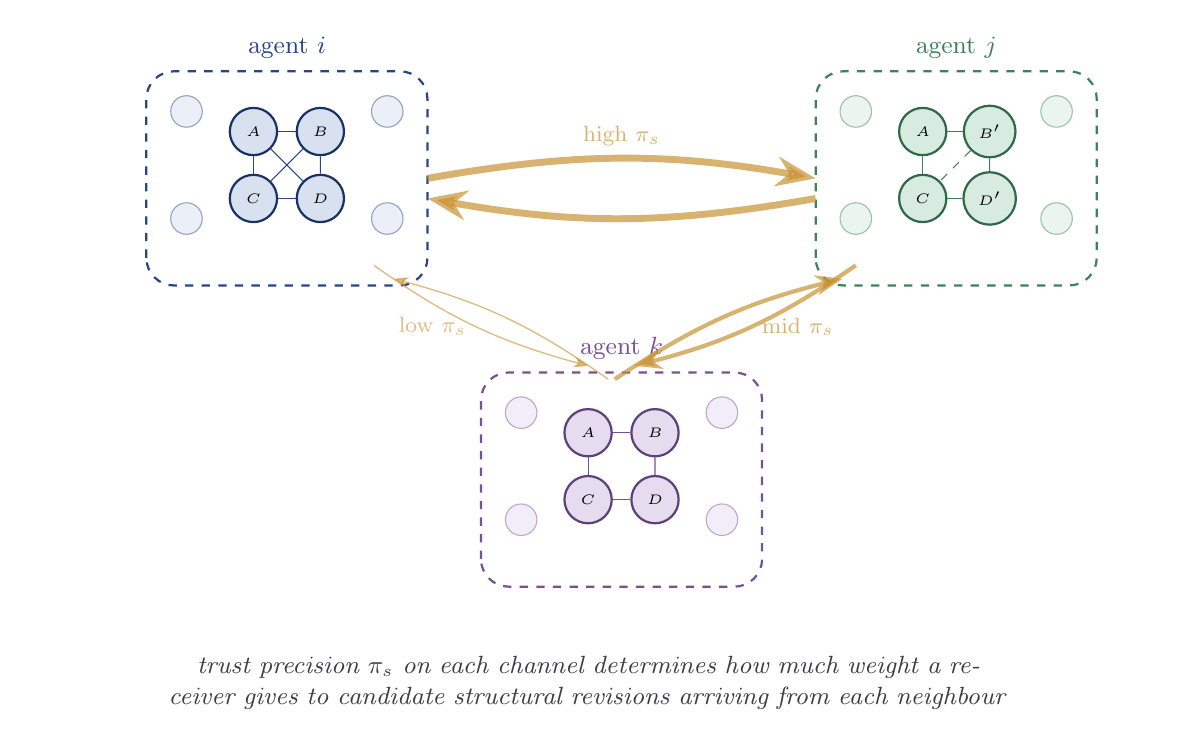
\begin{tikzpicture}[scale=0.85]

  % AGENT 1 - top left
  \begin{scope}[xshift=0cm, yshift=4cm]
    \draw[thick, coreblue, dashed, rounded corners=10pt] (-1.6, -1.6) rectangle (2.6, 1.6);
    \node[font=\small, coreblue, anchor=south] at (0.5, 1.65) {agent $i$};

    % mini network
    \node[circle, draw=coredeep, thick, fill=softblue, minimum size=6mm, font=\tiny] (i1) at (0, 0.7) {$A$};
    \node[circle, draw=coredeep, thick, fill=softblue, minimum size=6mm, font=\tiny] (i2) at (1, 0.7) {$B$};
    \node[circle, draw=coredeep, thick, fill=softblue, minimum size=6mm, font=\tiny] (i3) at (0, -0.3) {$C$};
    \node[circle, draw=coredeep, thick, fill=softblue, minimum size=6mm, font=\tiny] (i4) at (1, -0.3) {$D$};
    \draw[coreblue] (i1) -- (i2);
    \draw[coreblue] (i1) -- (i3);
    \draw[coreblue] (i2) -- (i4);
    \draw[coreblue] (i3) -- (i4);
    \draw[coreblue] (i1) -- (i4);
    \draw[coreblue] (i2) -- (i3);
    \node[circle, draw=coreblue!50, fill=softblue!50, minimum size=4mm] at (-1, 1) {};
    \node[circle, draw=coreblue!50, fill=softblue!50, minimum size=4mm] at (2, 1) {};
    \node[circle, draw=coreblue!50, fill=softblue!50, minimum size=4mm] at (-1, -0.6) {};
    \node[circle, draw=coreblue!50, fill=softblue!50, minimum size=4mm] at (2, -0.6) {};
  \end{scope}

  % AGENT 2 - top right
  \begin{scope}[xshift=10cm, yshift=4cm]
    \draw[thick, paradigmB, dashed, rounded corners=10pt] (-1.6, -1.6) rectangle (2.6, 1.6);
    \node[font=\small, paradigmB, anchor=south] at (0.5, 1.65) {agent $j$};

    \node[circle, draw=paradigmB!80!black, thick, fill=softB, minimum size=6mm, font=\tiny] (j1) at (0, 0.7) {$A$};
    \node[circle, draw=paradigmB!80!black, thick, fill=softB, minimum size=6mm, font=\tiny] (j2) at (1, 0.7) {$B'$};
    \node[circle, draw=paradigmB!80!black, thick, fill=softB, minimum size=6mm, font=\tiny] (j3) at (0, -0.3) {$C$};
    \node[circle, draw=paradigmB!80!black, thick, fill=softB, minimum size=6mm, font=\tiny] (j4) at (1, -0.3) {$D'$};
    \draw[paradigmB] (j1) -- (j2);
    \draw[paradigmB] (j1) -- (j3);
    \draw[paradigmB] (j2) -- (j4);
    \draw[paradigmB] (j3) -- (j4);
    \draw[paradigmB, dashed] (j2) -- (j3);
    \node[circle, draw=paradigmB!50, fill=softB!50, minimum size=4mm] at (-1, 1) {};
    \node[circle, draw=paradigmB!50, fill=softB!50, minimum size=4mm] at (2, 1) {};
    \node[circle, draw=paradigmB!50, fill=softB!50, minimum size=4mm] at (-1, -0.6) {};
    \node[circle, draw=paradigmB!50, fill=softB!50, minimum size=4mm] at (2, -0.6) {};
  \end{scope}

  % AGENT 3 - bottom centre
  \begin{scope}[xshift=5cm, yshift=-0.5cm]
    \draw[thick, accentpurple, dashed, rounded corners=10pt] (-1.6, -1.6) rectangle (2.6, 1.6);
    \node[font=\small, accentpurple, anchor=south] at (0.5, 1.65) {agent $k$};

    \node[circle, draw=accentpurple!80!black, thick, fill=softpurple, minimum size=6mm, font=\tiny] (k1) at (0, 0.7) {$A$};
    \node[circle, draw=accentpurple!80!black, thick, fill=softpurple, minimum size=6mm, font=\tiny] (k2) at (1, 0.7) {$B$};
    \node[circle, draw=accentpurple!80!black, thick, fill=softpurple, minimum size=6mm, font=\tiny] (k3) at (0, -0.3) {$C$};
    \node[circle, draw=accentpurple!80!black, thick, fill=softpurple, minimum size=6mm, font=\tiny] (k4) at (1, -0.3) {$D$};
    \draw[accentpurple] (k1) -- (k2);
    \draw[accentpurple] (k1) -- (k3);
    \draw[accentpurple] (k2) -- (k4);
    \draw[accentpurple] (k3) -- (k4);
    \node[circle, draw=accentpurple!50, fill=softpurple!50, minimum size=4mm] at (-1, 1) {};
    \node[circle, draw=accentpurple!50, fill=softpurple!50, minimum size=4mm] at (2, 1) {};
    \node[circle, draw=accentpurple!50, fill=softpurple!50, minimum size=4mm] at (-1, -0.6) {};
    \node[circle, draw=accentpurple!50, fill=softpurple!50, minimum size=4mm] at (2, -0.6) {};
  \end{scope}

  % Trust channels between agents - thick = high precision, thin = low
  \draw[->, line width=2.5pt, accentamber, >=Stealth, opacity=0.7]
    (2.6, 4) to[bend left=10] node[midway, above, font=\footnotesize, sloped] {high $\pi_s$} (8.4, 4);
  \draw[<-, line width=2.5pt, accentamber, >=Stealth, opacity=0.7]
    (2.6, 3.7) to[bend right=10] (8.4, 3.7);

  \draw[->, line width=0.5pt, accentamber, >=Stealth, opacity=0.6]
    (1.8, 2.7) to[bend right=10] node[midway, left, font=\footnotesize] {low $\pi_s$} (5, 1.2);
  \draw[<-, line width=0.5pt, accentamber, >=Stealth, opacity=0.6]
    (2.1, 2.5) to[bend left=10] (5.3, 1.0);

  \draw[->, line width=1.5pt, accentamber, >=Stealth, opacity=0.7]
    (9, 2.7) to[bend left=10] node[midway, right, font=\footnotesize] {mid $\pi_s$} (5.7, 1.2);
  \draw[<-, line width=1.5pt, accentamber, >=Stealth, opacity=0.7]
    (8.8, 2.5) to[bend right=10] (5.4, 1.0);

  % bottom label
  \node[font=\small\itshape, anchor=north, text width=14cm, align=center, text=darkgrey]
    at (5, -3) {trust precision $\pi_s$ on each channel determines how much weight a receiver gives to candidate structural revisions arriving from each neighbour};

\end{tikzpicture}
\end{center}

\noindent\textit{\textcolor{notegrey}{Each agent carries a full structured paradigm rather than a scalar belief. Agent $i$ and agent $k$ share the same structure (both blue/purple variants); agent $j$ has a structurally different paradigm (note the primed nodes $B'$, $D'$ and the different edge between $B'$ and $C$). The trust channels between agents are weighted by source precision $\pi_s$, drawn with proportional line thickness. This is the figure that makes the bubble-versus-chamber distinction natural: $i$ and $j$ have a high-$\pi_s$ channel (open to each other's structural revisions); $i$ and $k$ are connected but with low $\pi_s$ (chamber-style: edge present but precision near zero); and a missing edge between any two agents would be the bubble case (topological absence rather than precision suppression). This figure also shows where structural utility starts to matter at the population level: agents who attach high utility to their current structure will have low precision on channels carrying revisions to that structure, which is the network-level analogue of the individual-level motivated attention.}}

\newpage
%==============================================================
\section*{Notes on the figure set}
%==============================================================

\textit{The six figures together build a visual argument that the structural model is doing work the scalar model cannot.}

Figure 1 establishes that the paradigm is not a scalar. Figure 2 makes the carry-over property visible as cascading message propagation. Figure 3 shows that conservatism is derived from structural position rather than assigned. Figure 4 introduces BMR as continuous navigation through a precision space whose corners are discrete topologies. Figure 5 displays the central empirical contrast — sharp scalar cascade versus graded structural reorganisation — that distinguishes what the structural model predicts from what David's scalar simulations can produce. Figure 6 lifts the construction to the multi-agent setting, where trust precision on inter-agent channels carries candidate structural revisions rather than scalar belief mixtures.

\textit{Choices made.} Each figure prioritises one conceptual move. Figure 5 is the headline result and would be replaced with actual simulation output in the published version. Figure 4 is the most abstract and may benefit from accompaniment by a small concrete example (e.g. ``here is what removing one edge looks like in the precision space''); I have not included that here because it would clutter the diagram, but it is worth considering as supplementary material. Figure 6 is dense and may benefit from being split into two figures (one for the structural exchange, one for the trust-precision-versus-topology distinction) depending on how much room the paper has.

\textit{What is not in the figures.} I have not drawn the active-inference policy explicitly — the expected free energy minimisation that couples attention and action. A figure for this would show the agent selecting a sampling action over belt nodes under a paradigm-dependent value function, but the figure tends to be busy and the maths in the body of the paper carries the work more cleanly than a diagram could. If the paper needs a seventh figure for the policy, the natural form is a decision diagram showing two candidate sampling actions evaluated under expected free energy with the structural utility term tilting toward the paradigm-consistent option.

\textit{What needs to be done next.} The figures are sketches; they need (1) accurate equation references once the model file is consolidated, (2) consistent colour scheme with whatever the rest of the paper uses, (3) careful adjustment of node positions and edge thicknesses for visual clarity at publication scale, and (4) replacement of Figure 5 with actual simulation output once the structural model is implemented and the empirical signature is observed.

\end{document}